This section shows the tools we use to benchmark the databases in a real environment, which databases we choose to use, and why, and which energy measurement tools we use to collect CPU, primary and secondary storage energy, and the overall system design we use.

\subsection{Benchmark Tools}


\subsection{Benchmark}

Benchmarks are techniques that seek to collect and compare a wide variety of activities, to achieve the best result, an objective criterion for determining which practice or software is superior in certain scenarios that the user who
is doing the simulation built. An example of popular questions is "Which domain is the best system?”. The SPECCpu benchmark ~\cite{henning2006spec}, for instance, addresses the question, "What is the best CPU?" "and the \gls{tpcc} ~\cite{council2010tpc} responds to the question, "What is the best OLTP database system?” ~\cite{benchmarkchen}.

For ~\citeauthor{gray} a domain-specific benchmark must meet four important criteria to be a useful benchmark. It must be:

\begin{itemize}
    \item \textbf{Relevant:} In performing typical operations within that problem domain, it must measure the peak performance and price/performance of systems. 
    \item \textbf{Portable:} It should be easy to implement the benchmark on many different systems and architectures.
    \item \textbf{Scaleable:}  The benchmark should apply to computer systems small and large. As computer performance and architecture evolve, it should be possible to scale the benchmark up to bigger systems and to parallel computer systems.
    \item \textbf{Simple:} The benchmark must be understandable, otherwise credibility will be lacking.
\end{itemize}



%For conducting the measurements of the energy spent, we need first a benchmark tool that can be a load generator system that can emulate a real environment in \gls{dbms}.

\subsubsection{TPC Benchmark C}
\glsfirst{tpcc} is an \gls{oltp} workload~\cite{council2010tpc}. It is a mixture of read-only and update intensive transactions that simulate the activities found in complex \gls{oltp} application environments. It does so by exercising a breadth of system components associated with such environments, which are characterized by:

\begin{itemize}
    \item The simultaneous execution of multiple transaction types that span a breadth of complexity
    \item On-line and deferred transaction execution modes
    \item Multiple on-line terminal sessions
    \item Moderate system and application execution time
    \item Significant disk input/output
    \item Transaction integrity (\gls{acid} properties)
    \item Non-uniform distribution of data access through primary and secondary keys
    \item Databases consisting of many tables with a wide variety of sizes, attributes, and relationships
    \item Contention on data access and update
\end{itemize}

While these specifications express implementation in terms of the relational data model with a traditional locking framework, any commercially available \gls{dbms}, database servers, file systems, or other data repositories offering a functionally equivalent implementation can be used to implement the database.

\gls{tpcc} uses metrics and terminology that are similar to other benchmarks originating from the TPC or others. In no way does this similarity in terminology imply that the results of \gls{tpcc} are comparable to other benchmarks. Other \gls{tpcc} results compliant with the same revision are the only benchmark results comparable to \gls{tpcc}.

The performance metric reported by \gls{tpcc} is a "business throughput" measuring the number of orders processed per minute. Multiple transactions are used to simulate the business activity of processing an order, and each transaction is subject to a response time constraint. The performance metric for this benchmark is expressed in \gls{tpmc}. 

\gls{tpcc} is accepted in the industry as the most credible transaction processing benchmark with a large body of results across all major hardware and database platforms. The highly tuned and optimized nature of the \gls{tpcc} configurations makes it the best candidate for study \gls{dbms} power consumption~\cite{powerconsumptiontppc}.

\subsubsection{HammerDB}



We decide to use HammerDB as it is a benchmark tool that can replicate the behavior of most cloud-based applications as a service, verify comprehensive performance and multiple metrics in a simple real-world environment on a virtual environment with virtual users.~\cite{hammerdb}.



HammerDB is an Open source tool and accepted tool to benchmark DBMS because of this there is a lot of studies that use and recommend HammerDB to test and/or compare different DBMS ~\cite{scalzo2018database,elgrablyanalise,knoche2016combining,benchmarkchen,ali2019persistent,yu2015design,koccak2018software,koccak2018software}. \citeauthor{elgrablyanalise} study use HammerDB to compare open-source DBMS performance like Mysql, MariaDB and Postgres \cite{elgrablyanalise}. Another study that uses Hammerdb is \citeauthor{knoche2016combining}~(\citeyear{knoche2016combining}) work that use hammerdb to test the Impact of Database Lock Contention in the \gls{tpcc} Benchmark scenario \cite{knoche2016combining}. As a final example, we have \citeauthor{koccak2018software}~(\citeyear{koccak2018software}) that use HammerDB on MySQL to have a dataset to use on his software energy consumption prediction~\cite{koccak2018software}. 


HammerDB is also used by all leading database and technology companies. It has been downloaded hundreds of thousands of times to more than 180 countries in the world and even some well know companies such as Oracle, IBM, Intel, Dell/EMC HPE, Huawei, Lenovo, and hundreds more~\cite{hammerdb}.



HammerDB is a tool that can emulate a \gls{tpcc} scenario 
and through \gls{oltp} workloads it sets up a company's sales processing environment. It reduces the testing costs by simplifying the \gls{tpcc} rules, can be modified and run on a custom environment. The above factors result in a low-cost solution, rapid deployment, and personalized benchmark test \cite{benchmarkchen,elgrablyanalise,hammerdb}. 

 Since HammerDB implements a workload based on the \gls{tpcc} specification but does not implement a complete \gls{tpcc} benchmark specification, and because of that the transaction results from HammerDB can't be compared with the official \gls{tpcc} benchmarks published. HammerDB workloads generate 2 statistics. \gls{tpm} is the transactional measurement of the specific database typically defined as the number of user commits plus the number of user rollbacks. \gls{tpm} values are database-specific cannot be compared between different types of databases. The \gls{nopm} value, on the other hand, is a performance metric independent of any particular database implementation and is the recommended primary metric to use~\cite{hammerdb}.

HammerDB currently supports Oracle, SQL Server, Db2, TimesTen, MySQL, MariaDB, PostgreSQL, Greenplum, Postgres Plus Advanced Server, Redis, and more, and can run on a variety of operating systems, being an elastic and heterogeneous tool~\cite{benchmarkchen}.

Another reason we choose him was that HammerDB is used for automated software testing \cite{hammerdb} so we can configure how many times the HammerDB will run and how many virtual users that he will use and for how long it will run, providing at the end of every execution the \gls{tpm} and the \gls{nopm}. With these numbers and the energy spent, we can have ample information to answer the RQ2, and with an adjustable number of users, it can assist in the RQ3.



\subsection{Database Under Test}

After having Relational databases dominated the software industry for a long time, the advantage that they have is of being well structured with strong data store structures, concurrency control and interfaces. 
%MELHOR ligação entre as frases

We decide to choose the 3 of the most trendy relational databases that Hammerdb could support and one non-relational database.~\cite{DBR}.
The DBMS chosen where:
\begin{itemize}
  \item Mysql : explicar e Motivos a frente
  \item Postgres : explicar e Motivos a frente
  \item MariaDB : explicar e Motivos a frente
  \item Redis : explicar e Motivos a frente
\end{itemize}

For consistency reasons, we use the TPC-C model provided by hammerdb and apply to every database. 
%nao tenho acerteza se devo por esta parte

In the TPC-C database model, a wholesale parts supplier operates out of a number of warehouses and their associated sales districts. 
In this model, each warehouse has to supply ten sales districts, and each district serves three thousand customers. An operator in a sales district can choose one of the five operations or transactions provided by the order-entry system of the Business at any time.  The frequency of the individual transactions, like the transactions themselves, is based on practical scenarios.

For simplification reasons we decide to play this configuration to our model:

\input{tables/databaseconfig}

%TPPC WEBSITE REF???

Another cautions we did to have more reliable results was to mount the DBMS on this disk because we don't want the operating system interfering on our measurements.


\subsection{Energy Measurement Tools}
if we want to analyze energy consumption, We must be able to obtain energy readings. For that, we will need two tools, one for CPU and DRAM, and secondary memory.

\subsubsection{\textbf{CPU and Primary storage}}

   Intel’s \gls{rapl} is a tool to measure the energy on \gls{cpu} and primary storage (\gls{dram}). Here it will explain how it got introduce, how it works, and the limitations it has.
	
	\gls{rapl} is a well-known and accepted interface for measuring the power consumption of a computer system. Various studies used this interface as a measuring tool, and others review Intel \gls{rapl} measurements in terms of accuracy, performance, granularity, usability ~\cite{raplpref,raplpref2}.
	

	Intel introduced \gls{rapl} on they compilers in the architecture of the Intel Sandy Bridge, and since the first appearance, it has been evolving in the newer architectures. \gls{rapl} has \gls{msr} that aren't part of the architecture of the processor but address power values required for energy consumption management ~\cite{raplpref,intel64and,portela2016}.
	
	
    The mains functionalities of the \gls{rapl} are to measuring the energy consumption on the \gls{cpu} and primary storage and also to limit the energy consumption on the components mentions. In the context of this research, we won't use the last functionality, as it does not fit in the context of this study ~\cite{raplpref,raplpref2,intel64and}.
	
	
	The \gls{rapl} does not measurements energy based on an analog energy meter because energy consumption is estimated through the analysis of various hardware performance counters, temperature sensors, leakage energy, and IO models.  Registers reserved for energy readings are updated approximately every millisecond (1kHz) ~\cite{energypapi,portela2016}.

    \begin{figure}[ht!]
    \centering
    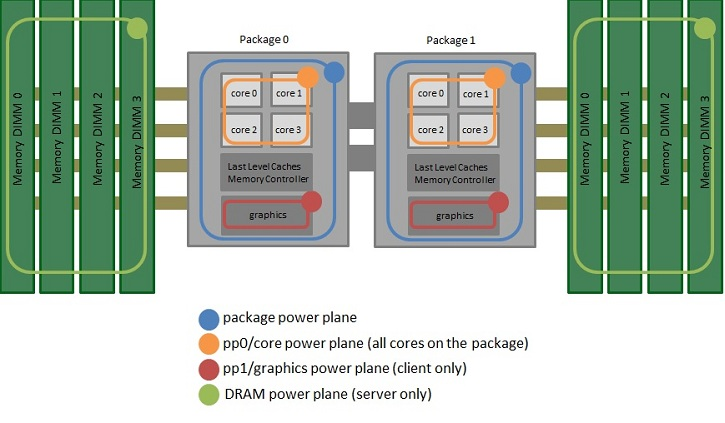
\includegraphics[width=\linewidth]{Chapters/images/power_domains2.jpg}  \caption{Intel’s \gls{rapl} Power Domain.}
    \label{fig:powerdomain}
    \end{figure}
    
    We can check the different power domains supported by \gls{rapl} in figure \ref{fig:powerdomain}. Each power domain has a different  \gls{msr}  and reports the domain's energy consumption, allowing us to limit that domain's power usage over a specified time. Each domain represents distinct physical component sets, currently, these are: 
    
    \begin{itemize}
        \item \textbf{Package}: the package domain refers to the package's energy consumption of the entire socket, including the core and uncore components energy ~\cite{intel64and}.
        \item \textbf{PP0/Core Power Plane 0}: This domain measurement the energy consumption of all processors socket~\cite{intel64and,portela2016}.
            \item \textbf{PP1/Graphics Power Plane 1}: This domain measures the energy consumed by all processors in a \gls{gpu}.
        \item \textbf{DRAM}: This Domain refers to the energy consumption of random access memory (RAM)~\cite{intel64and,portela2016}.
        \item \textbf{Psys}: Intel \textit{Skylake} has introduced a new \gls{rapl} Domain named PSys. It monitors and controls the thermal and power specifications of the entire SoC and it is particularly useful when the source of power consumption is neither the \gls{cpu} nor the \gls{gpu} \cite{raplpref}.
    \end{itemize}
    For multi-socket server systems, each socket reports its own \gls{rapl} values \cite{raplpref}.
    
    There are some distinctions between the list of available domains, depending on the type of platform. The available domains on platforms intended for the client are Package, Power Plane (PP) 0, and PP1. On the other hand, the Package, PP0, and \gls{dram} domains are available on the Platform intended for Servers \cite{raplpref2}.
    In the Table \ref{tab:rapltable} presents an overview of \gls{rapl} domains supported by different processor model.
% Please add the following required packages to your document preamble:
% \usepackage{multirow}
\begin{table}[H]
\centering
\caption{RAPL power domains supported by different models}
\begin{tabular}{|c|c|c|c|c|c|}
\hline
\multirow{ }{Model }{} & \multicolumn{5}{c|}{Power domain supported} \\ \cline{2-6} 
                       & PKG    & PPO    & PP1    & DRAM    & PSYs   \\ \hline
Sandy Bridge           & YES    & YES    & YES    & NO      & NO     \\
Sandy Bridge-EP        & YES    & YES    & NO     & YES     & NO     \\
Haswell                & YES    & YES    & YES    & YES     & NO     \\
Haswell-EP             & YES    & NO     & NO     & YES     & NO     \\
Skylake                & YES    & YES    & YES    & YES     & YES*   \\ \hline
\end{tabular}
\label{tab:rapltable}
\newline
*Not All Skylake versions support PSys

\end{table}

    The MSR interfaces available in each of the domains mentioned are the following:
\begin{itemize}

    \item \textbf{Power Limit}: interface serves to specify the time interval and the limit of energy to be consumed~\cite{raplpref2,portela2016}. 
\item \textbf{Energy Status}: This interface provides the energy consumed. The register reports the actual power used by the domain. This interface is read-only. 
\item\textbf{Perf Status}: This interface is optional and provides the effects of restrictions used~\cite{intel64and,portela2016}.
\item \textbf{Power Info}: This interface is optional and presents the information for a given domain (Power, Energy, etc.)~\cite{portela2016}.
\item \textbf{Policy}: This Interface is optional and it allows defining control policies for energy to distribute costs, that is, to balance the power consumed between domains subdomains ~\cite{raplpref2}. 
\end{itemize}

With all this information we can conclude that the largest domain we can get on \gls{rapl} is with this equation:

\begin{equation}
E_{PPO} + E_{PP1} <= E_{Packgage}
\end{equation}$
$

To gather results, we develop software in C, that is running in parallel with the task we want to measure. On the listing \ref{lst:raplcode} , is a example of the code we made.

    
    \begin{lstlisting}[ caption={ Exemple of reading RAPL energy in C},label={lst:raplcode},language=C,
    basicstyle=\tiny, %or \small or \footnotesize etc.
]
void rapl_after(FILE * fp , int core){ 
  int fd;
  long long result;
  fd=open_msr(core);

  result=read_msr(fd,MSR_PKG_ENERGY_STATUS);
  package_after=(double)result*energy_units;
  fprintf(fp,"%.6f , ",package_after-package_before);  // PACKAGE

  result=read_msr(fd,MSR_PP0_ENERGY_STATUS);
  pp0_after=(double)result*energy_units;
  
  fprintf(fp,"%.6f , ",pp0_after-pp0_before);    // CORE

  if ((cpu_model==CPU_SANDYBRIDGE) || (cpu_model==CPU_IVYBRIDGE) ||
	(cpu_model==CPU_HASWELL)) {
     result=read_msr(fd,MSR_PP1_ENERGY_STATUS);
     pp1_after=(double)result*energy_units;
     fprintf(fp,"%.6f , ",pp1_after-pp1_before);     // GPU
  }
  else fprintf(fp,"  , ");   
  
  if ((cpu_model==CPU_SANDYBRIDGE_EP) || (cpu_model==CPU_IVYBRIDGE_EP) ||
	(cpu_model==CPU_HASWELL)) {
     result=read_msr(fd,MSR_DRAM_ENERGY_STATUS);
     dram_after=(double)result*energy_units;
     fprintf(fp,"%.6f , ",dram_after-dram_before);     // DRAM
  }
  else fprintf(fp,"  , "); }
\end{lstlisting}


    The \gls{msr} driver must be enabled for direct MSR access with \textit{/dev/cpu/*/msr} command, and read access permission must be set for the driver. Reading \gls{rapl} domain values directly from \gls{msr} requires the \gls{cpu} model to be detected and the \gls{rapl} energy units read before reading the consumption values of the \gls{rapl} domains ~\cite{raplpref,energypapi}. Once the \gls{cpu} model is detected, the \gls{rapl} domains can be read per package of the \gls{cpu} by reading the corresponding “MSR status” register  ~\cite{raplpref,intel64and}.

    
\subsubsection{\textbf{Secondary Storage}}

To benchmark the energy consumption on disk storage, we had to choose between indirect methods or direct methods.

%The Indirect methods consist of estimating the energy base how much time he spent in which state and how much the seeks, reads, and writes, and knowing much which operation costs and how much energy he spent every time he which is every state. With that knowledge, we can estimate how much energy consumption during that time. This approach produces good results, but since all energy is an estimate, this procedure including an error margin on the results.

%The other approach is the direct method by using external hardware, this method consists of measuring Electric Potential Difference on the disk. This method is a lot precise since the results are real, but the downsize it is that have an impact on the overall performance, this impact it only notices on a big scale~\cite{portela2016}.

It was opt-in for a instant power measurement approach because this was the simplest and sufficient solution to achieve the objectives intended of reading, constantly and automatically the energy consumption on the secondary storage ensuring that our results are precise and reliable and since our measurements are on a small scale it doesn't have an impact on the overall systemy~\cite{portela2016}.

Since it is necessary data handling on our behalf and because we need to store energy spent, a normal ammeter won't do the work. Thus to gather our measurements we choose to use an Arduino Uno with a current sensory~\cite{portela2016}.

The SATA cable is responsible for distributing energy to the disk and data exchange between the secondary memory and the computer. So to get the energy on the disk we must connect the current sensor to the connection of the SATA cable that is responsible for distributing energy~\cite{portela2016}.

The current sensor we opt-in was the Low Current Sensor Breakout. This current sensor is marketed by SparkFun and can measure the current regardless of whether the signal is continuous or alternating. The sensor is also accompanied by an operational amplifier phase to control the gain, which can measure lower currents more precisely ~\cite{portela2016}.

\begin{figure}[H]
  \caption{Scheme of connections between Sata cable, current sensor and Arduino used to measurement secondary storage.}
  \centering
  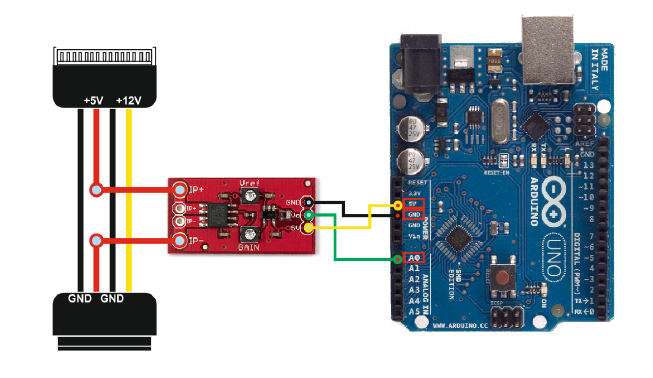
\includegraphics[width=\linewidth]{Chapters/images/arduino.png}
\end{figure}

Also, an Arduino UNO was used to read the analog voltage presented by the sensor and communicate these values to the computer connected to it through the serial port. For this, we had to develop a program for the Arduino that would get take constant readings at the analog voltage and send them every 0.1 seconds. 

  \begin{lstlisting}[ caption={ Arduino source code for reading the analog signal from the current sensor},label={lst:arduinocode},language=C,
    basicstyle=\small
]
void loop() {
  /* Initialization */
  float average_a0 = 0; // Raw reading from pin
  float voltage = 0; // Voltage in V
  float current = 0; // Current in A
  float wattage = 0; // Wattage in W
  float power = 0; // Power in J
  /* Average loop */
  for(int i = 0; i < n_reads ; i++) {
    average_a0 += analogRead(sensorPin_0);
    delay(loop_delay);  }
  /* Formula based computations */
  average_a0 /= n_reads;
  voltage = (average_a0 / 1024.0) * 5;
  current = current_eq(voltage);
  wattage = voltage * current;
  power = wattage * interval;
  Serial.println(power, 3);
  Serial.flush();}

\end{lstlisting}


Following the code on the listing \ref{lst:arduinocode}, the reading is made every millisecond and then is made the average of the last one hundred milliseconds, which is finally sent to the computer system connected to the Arduino.



\subsection{Overall Design}

To get precise and correct measurements, at the start of every benchmark that Hammerdb does to any Database, the Arduino and RAPL start in different and synchronized threads and start their executions simultaneously and only ending when Hammerdb it is over, as we can see in figure \ref{fig:arch}.

\begin{figure}[H]
  \centering
    \caption{Architecture Design}
  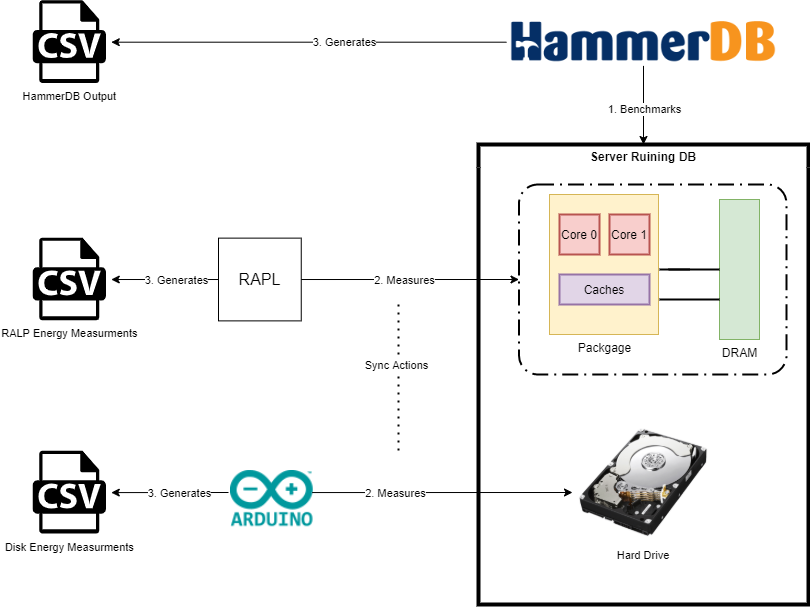
\includegraphics[width=\linewidth]{imagens/arquitetura.png}
  \label{fig:arch}
\end{figure}


To do the sync actions, we had to create a program that would start the Arduino and RAPL as differents threads, that only start at the beginning of HammerDB execution, and the end gathers the data obtain from the measurements tools and write in a CSV file.








